\documentclass[4pt,usenames,dvipsnames,aspectratio=169,table]{beamer}
%\usetheme{cern}
\usetheme{cernomc}

% Beamer Setup ---
\setbeamercovered{transparent=5} 
\setbeamertemplate{navigation symbols}{} 

\AtBeginSection{%
	\begin{frame}[noframenumbering]{Outline}
	\tableofcontents[currentsection]
	\end{frame}
}

% Imports ---
\usepackage[utf8]{inputenc}
\usepackage{amsmath}
\usepackage{amsfonts}
\usepackage{amssymb}
\usepackage{unicode-math}
\usepackage{mathtools}
\usepackage{bm}  % bold math
\usepackage{graphicx}
\usepackage{grffile}  % filenames with dots 
\usepackage{fontawesome5}
\usepackage{tikz}
\usepackage{hyperref}
\usepackage{siunitx}
\usepackage{booktabs}
\usepackage{multirow}
\usepackage{caption}
\usepackage[absolute,overlay]{textpos}

\usepackage{fontspec}
\usefonttheme{serif}
%\setmainfont{STIX Two Text}
%\setmathfont{STIX Two Math}
\setmainfont{TeX Gyre Bonum}
\setmathfont{TeX Gyre Bonum Math}


% some shenanigans -------------------------------------------------------------
\newcommand{\highl}[1]{\textbf{#1}}
\definecolor{RunTwored}{RGB}{200,0,0}
\definecolor{APJgreen}{RGB}{20,150,0}
\definecolor{SbSorange}{RGB}{240,150,0}
\newcommand{\we}{\cellcolor{blue!20!white}}
\newcommand{\ho}{\cellcolor{red!20!white}}

% highly illegal!
\newcommand{\faSunrise}{
\includegraphics[width=1em]{sunrise.png}}


% Meta -------------------------------------------------------------------------
\author[OMC]{%
Andreas Wegscheider on behalf of the OMC team:\\%
\small
T.~Persson,  F.~Carlier, A.~Costa~Ojeda, J.~Dilly, H. Garc\'ia Morales, V.~Ferrentino, 
 E.~Fol, M.~Hofer, E.J~Høydalsvik, J.~Keintzel, M.~Le~Garrec, E.H.~Maclean,    
 L.~Malina, F.~Soubelet, R.~Tom\'as, L.~Van Riesen-Haupt and A.~Wegscheider, CERN, Geneva, Switzerland \\
  J. Cardona, Universidad Nacional de Colombia\\[1em]
% hacky, I know ...
\centering%

\includegraphics[width=3cm]{OMC_logo_original.pdf}%
}
\title[LHC 2022]{LHC Commissioning 2022}
\logo{} 
\titlegraphic{}
\institute{CERN}
\date[09.06.22]{09.06.2022}
\subject{} 

% Document ---------------------------------------------------------------------
\begin{document}

\begin{frame}
    \titlepage
\end{frame}


\begin{frame}{Full Outline}
\tableofcontents
\end{frame}

\section{OMC Shifts}

\begin{frame}{Shift Schedule }

%\textbf{note:} this is just to collect now, will be cleaned for presentation

\begin{minipage}{0.45\linewidth}
\small
\begin{tabular}{ll|ll|ll}
    \multicolumn{2}{c}{April}
    &\multicolumn{2}{c}{May}
    &\multicolumn{2}{c}{June}\\
%date & actual            & date & actual          & date & actual            \\
\we 23.  & \we\faSunrise \faSun &     02.   &    \faSun \faMoon  &     03.   &    \faSun \faMoon    \\
\we 24.  & \we\faSun \faMoon    &     04.   &    \faSunrise      & \we 04.   & \we\faSun \faMoon    \\
    25.  &    \faSun            & \we 08.   & \we\faMoon         & \ho 06.   & \ho\faSunrise        \\
    26.  &    \faSun            &     09.   &    \faMoon         &           &                      \\
    27.  &    \faMoon           &     10.   &    \faMoon         &           &                      \\
    28.  &    \faMoon           & \we 21.   & \we\faMoon         &           &                      \\
         &                      & \we 22.   & \we\faMoon         &           &                      \\
         &                      & \ho 26.   & \ho\faSun          &           &                      \\
         &                      & \ho 27.   & \ho\faSun          &           &                      \\
         &                      & \we 28.   & \we\faSun \faMoon  &           &                      \\
         &                      & \we 29.   & \we\faSun          &           &                      \\
     \hline
 %    \multicolumn{2}{c|}{2(3)\faMoon / 6 }
 %    &\multicolumn{2}{c|}{5(7)\faMoon / 11}
 %    &\multicolumn{2}{c}{0(2)\faMoon / 3}
\end{tabular}\\
\footnotesize

\begin{tabular}{llll}
\faSun: day& \faMoon: night&
   \we weekend  & \ho holiday
\end{tabular}
\end{minipage}
\begin{minipage}{0.54\linewidth}
\normalsize

\begin{itemize}
    \item many shifts on holidays / weekends (11 out of 20)
    \item still many night shifts (7 pure and 12  with considerable nighttime out of 20 total)
    \item team of dedicated night owls
\end{itemize}

\end{minipage}

\end{frame}


\begin{frame}{Dedicated Collimation Sequence}

\begin{itemize}
    \item \highl{dedicated} collimation sequence to be trimmed in for \highl{OMC measurements}
    \item two settings: \highl{injection} and \SI{30}{cm} \highl{optics}
    \item \highl{automates} collimation setup
    \item crucial to get sufficient \highl{kick amplitude} at top energy
    \item no need to call collimation expert during night shift on a holiday
\end{itemize}

    
\end{frame}


\section{The Way to Top Energy}

% Injection --------------------------------------------------------------------


\begin{frame}{Injection optics}
    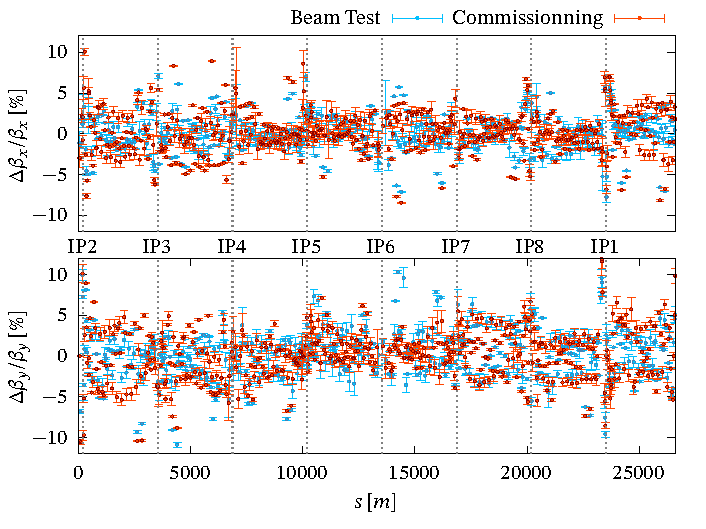
\includegraphics[width=0.49\linewidth]{images/beamtest/b1_bb.pdf}
    \hfill
    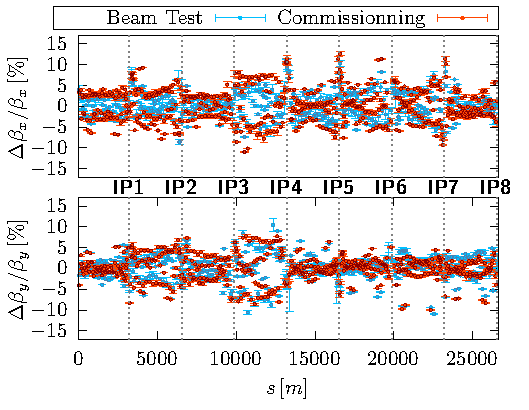
\includegraphics[width=0.49\linewidth]{images/beamtest/b2_bb.pdf}
    
    \begin{itemize}
        \item  Measured the injection optics with the corrections of \highl{2021 beam test}.
        \item Looks similar, \highl{no corrections} were re-calculated.
    \end{itemize}
\end{frame}


% Ramp -------------------------------------------------------------------------


\begin{frame}{Coupling in the Ramp}
    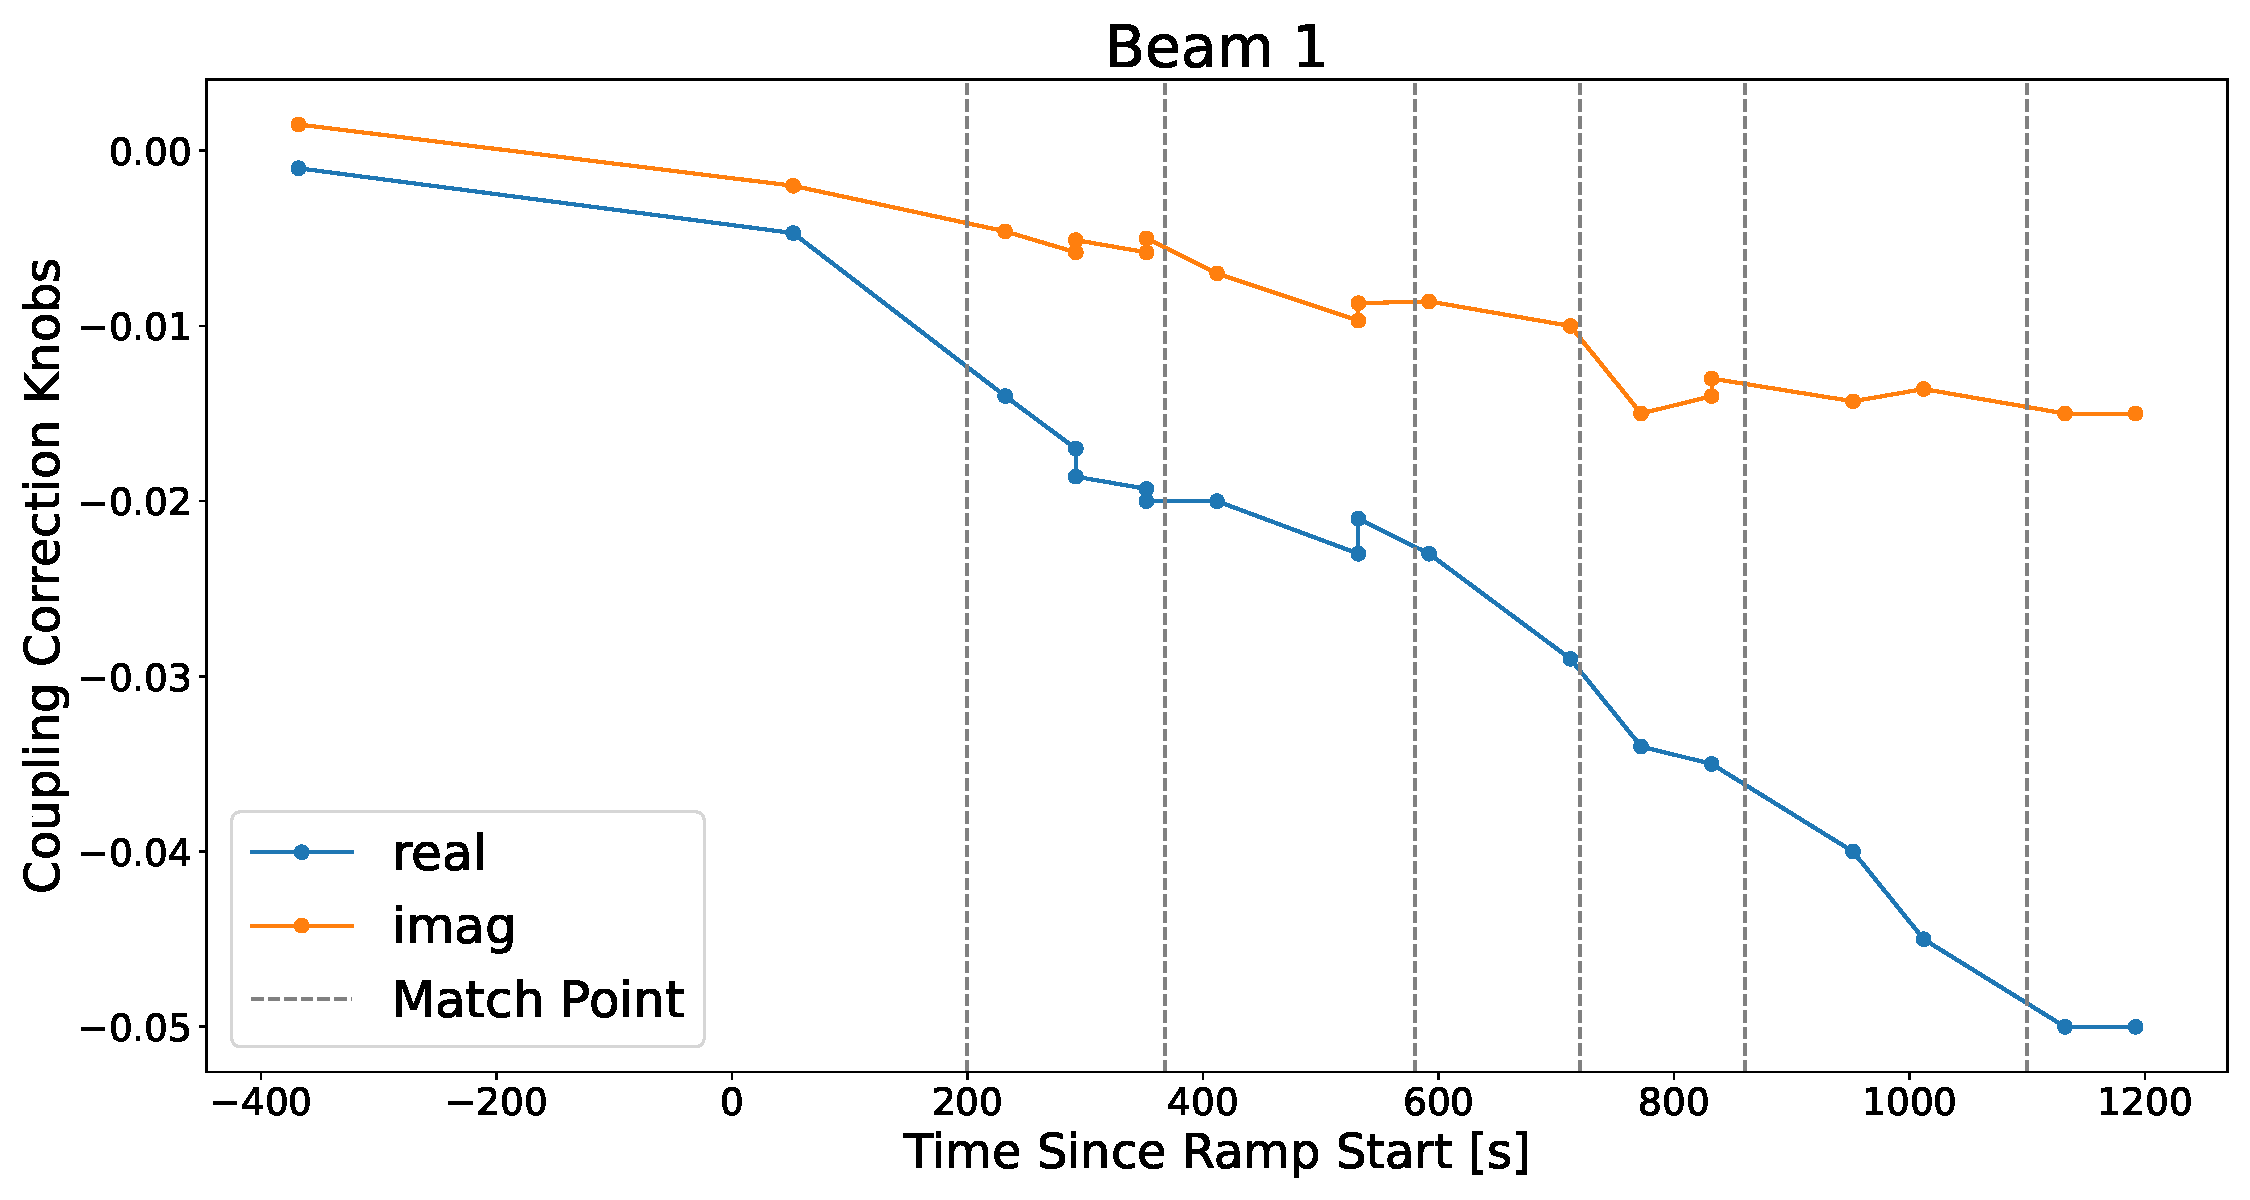
\includegraphics[width=0.49\linewidth]{images/ramp/B1_coupling_correction_knobs_in_ramp.pdf}
    \hfill
    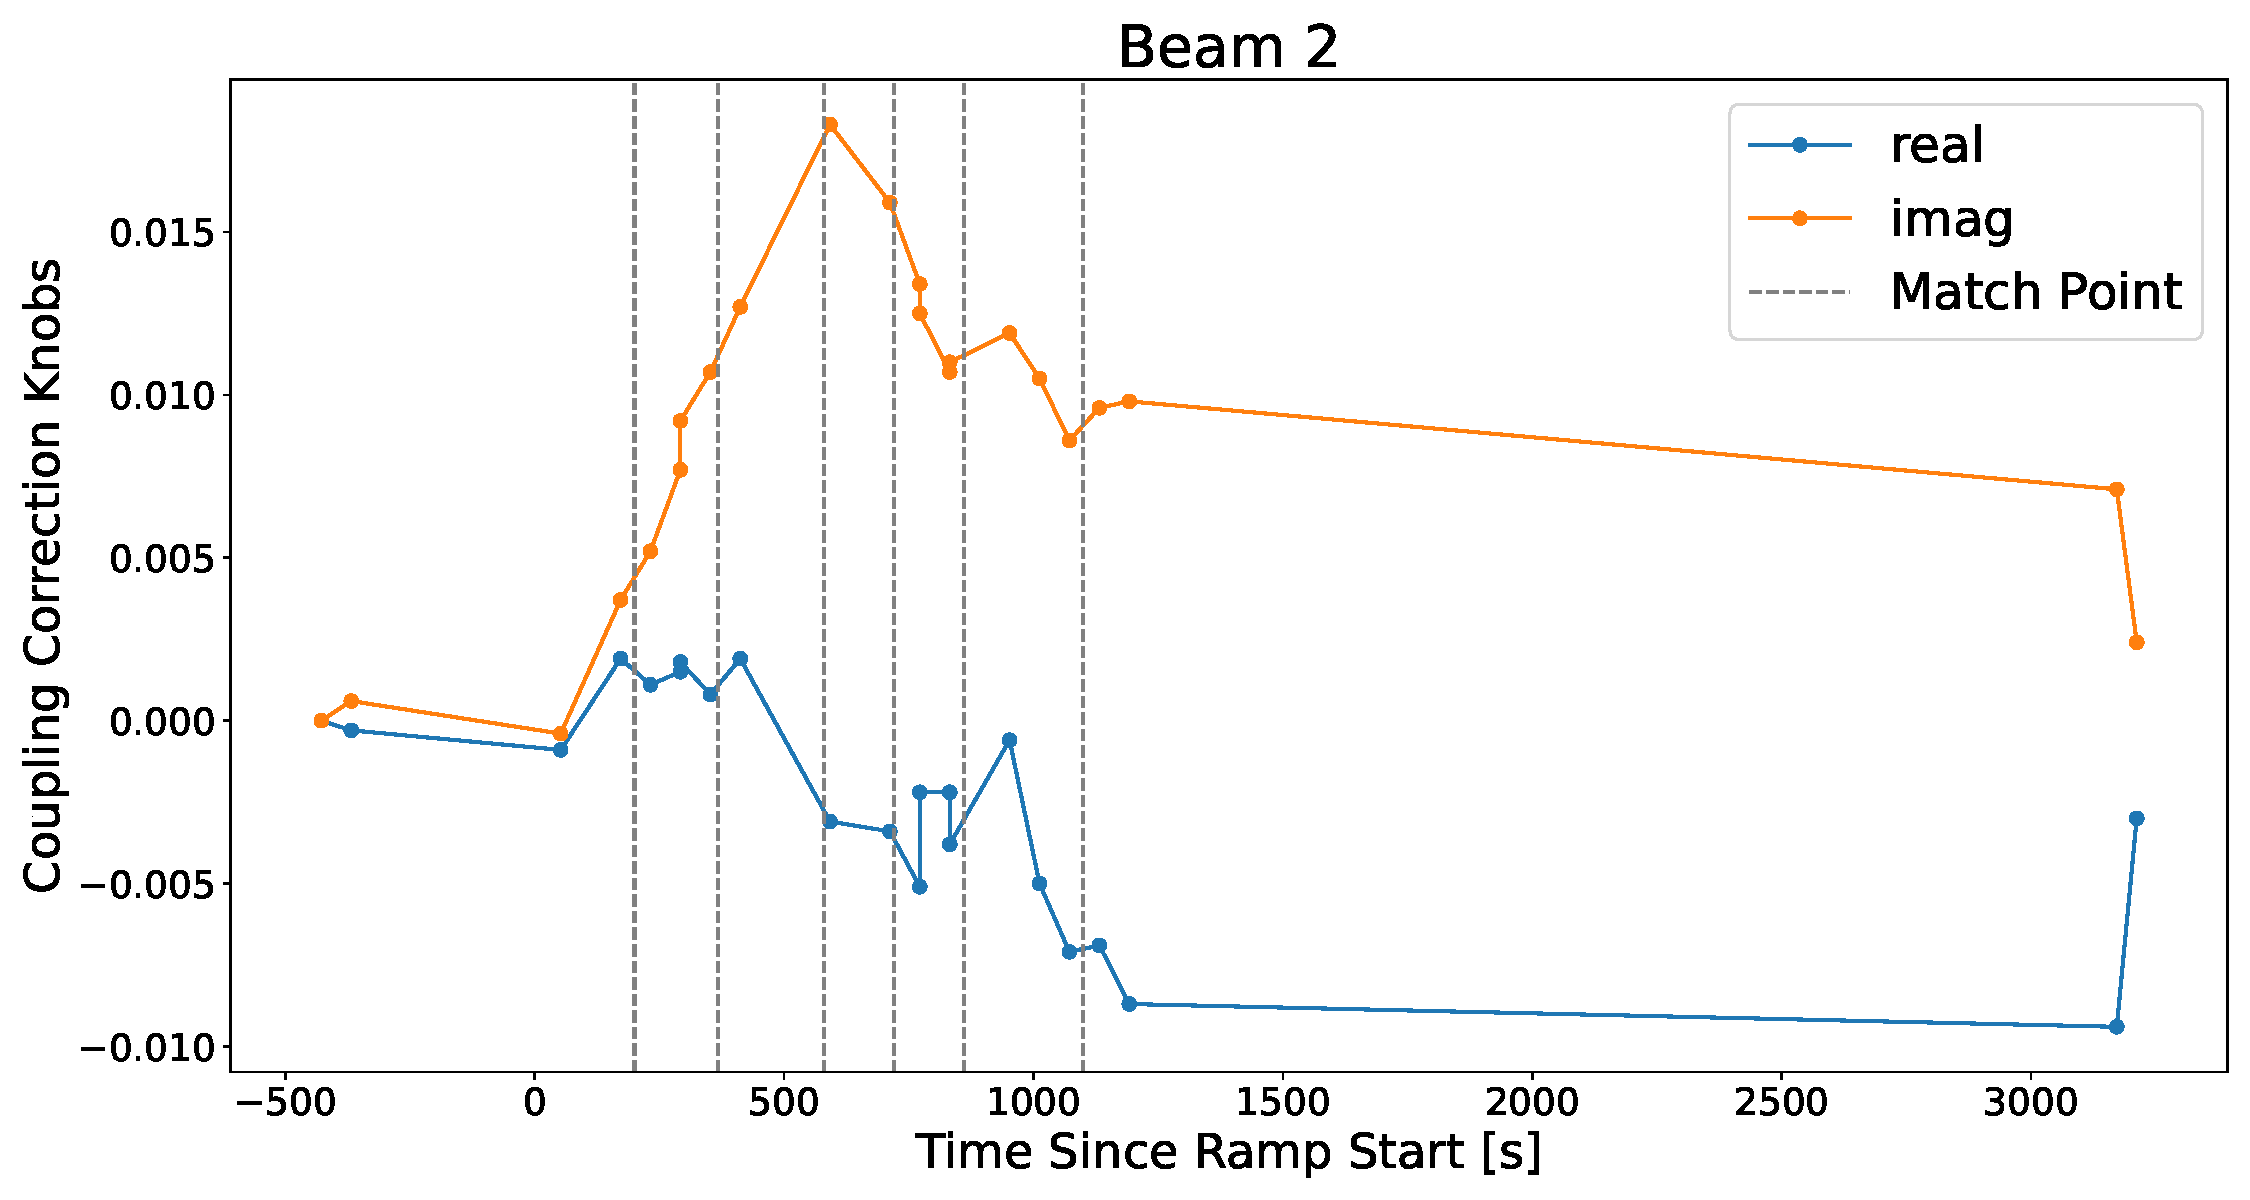
\includegraphics[width=0.49\linewidth]{images/ramp/B2_coupling_correction_knobs_in_ramp.pdf}
    
    \begin{itemize}
        \item %
            did \highl{manual coupling} measurement during the ramp because the coupling server
            \highl{failed to give} good results 
        \item %
            calculated \highl{coupling corrections} (verifying on the way that the selected model didn't deteriorate the calculations)
        \item %
            these were \highl{programmed in} to be applied during the next ramp
        \item %
            re-measure showed that we corrected \highl{$< 0.005$ at every pick-up point}
    \end{itemize}
\end{frame}


%% Flattop ---------------------------------------------------------------------
%
%
%\begin{frame}{Flattop, $\beta$=133\,cm}
%    
%    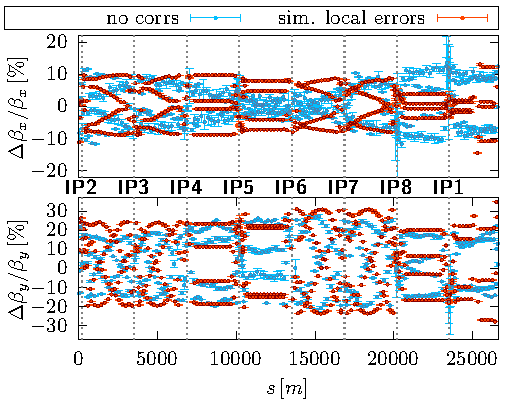
\includegraphics[width=0.49\linewidth]{images/flattop/b1_bb.pdf}
%    \hfill
%    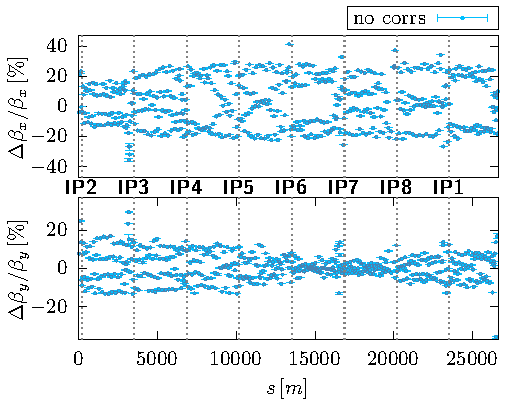
\includegraphics[width=0.49\linewidth]{images/flattop/b2_bb.pdf}
%    \begin{itemize}
%        \item measurements at \SI{6.8}{TeV} performed
%        \item errors within tolerances, no dedicated corrections
%    \end{itemize}
%    
%\end{frame}

\section{Squeeze}


\begin{frame}{30\,cm Optics -- record high $\beta$~beating}

    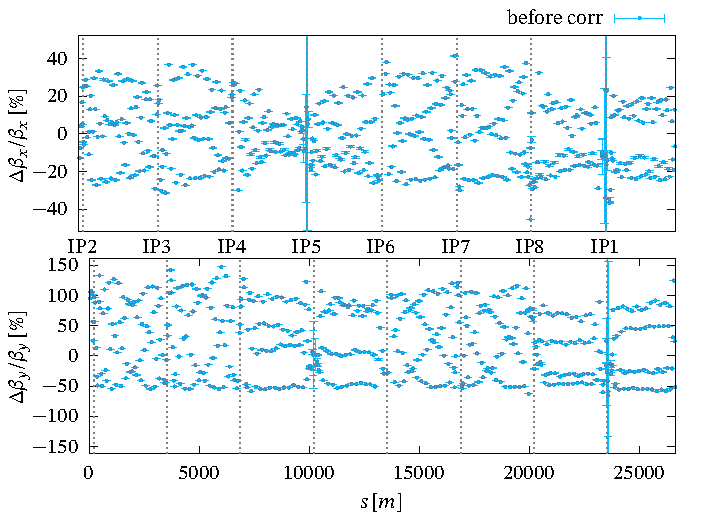
\includegraphics[width=0.49\linewidth]{images/squeeze/b1_recordhigh.pdf}
    \hfill
    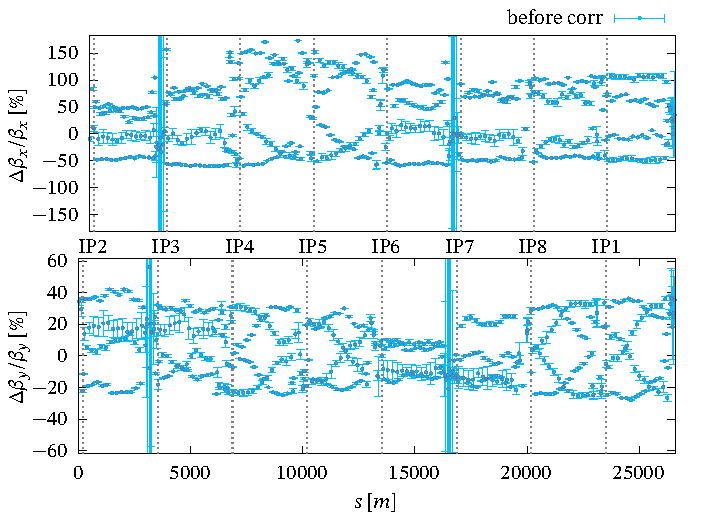
\includegraphics[width=0.49\linewidth]{images/squeeze/b2_recordhigh.pdf}
    
    \begin{itemize}
        \item peak $\beta$~beating of \textbf{150 \%}
        \item highest ever measured in the LHC
    \end{itemize}
    
\end{frame}


\begin{frame}{30\,cm Optics \only<2>{-- Beam~1}\only<3>{-- Beam~2}}
    \begin{center}
        \only<2>{
            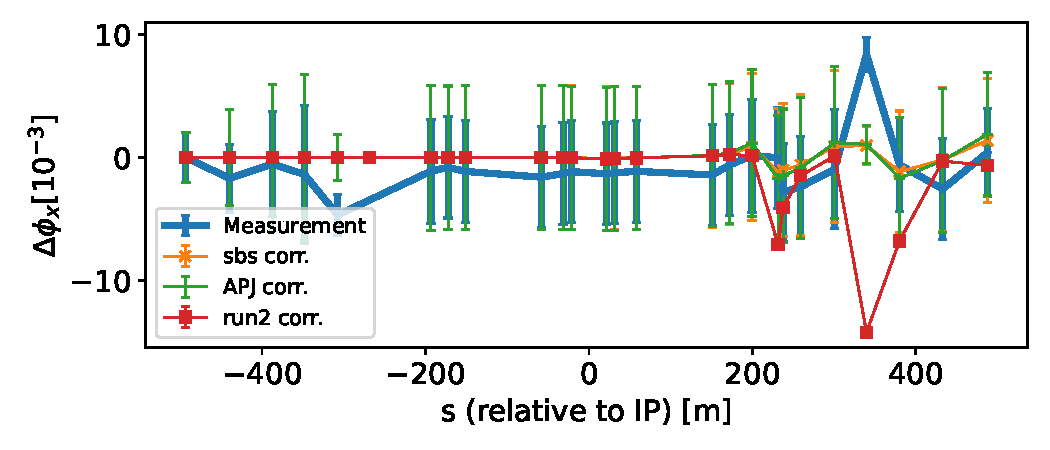
\includegraphics[width=0.4\linewidth]{images/flattop/beam1_x_IP1.pdf}
            \hspace{1cm}
            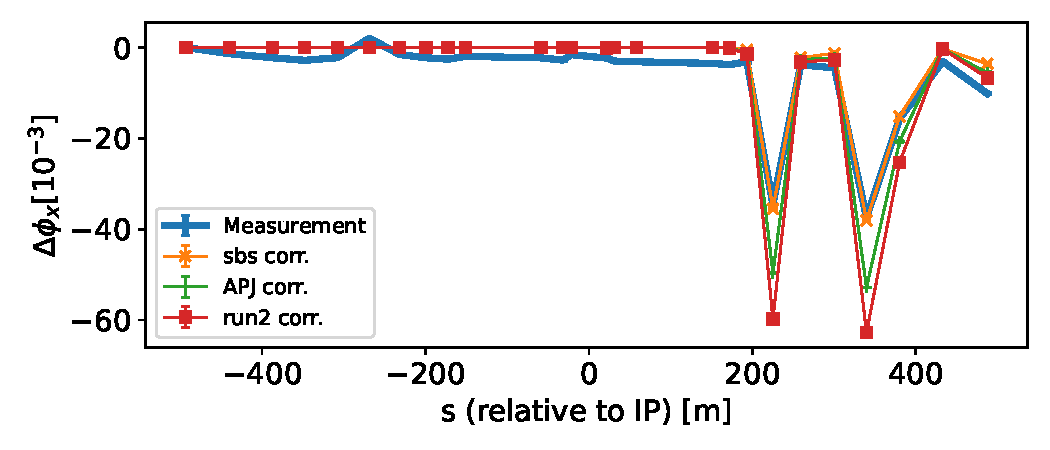
\includegraphics[width=0.4\linewidth]{images/flattop/beam1_x_IP5.pdf}
            \\
            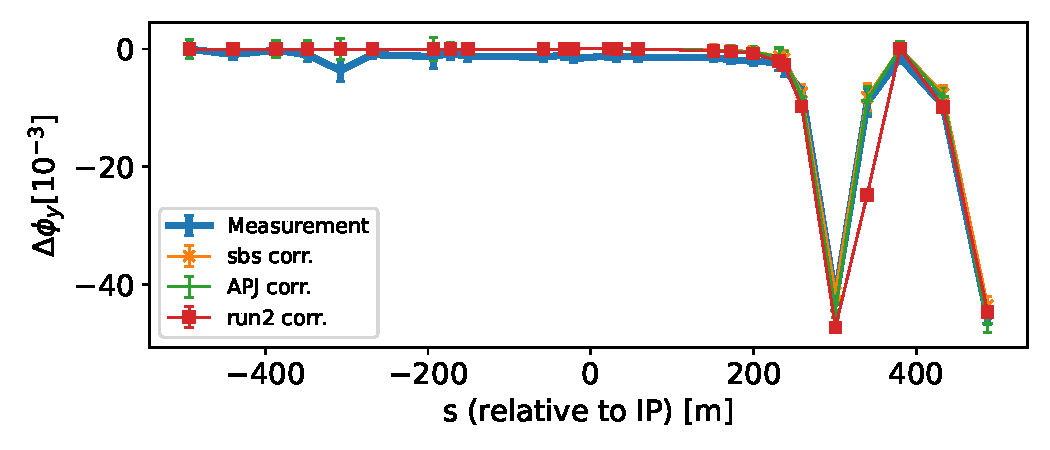
\includegraphics[width=0.4\linewidth]{images/flattop/beam1_y_IP1.pdf}
            \hspace{1cm}
            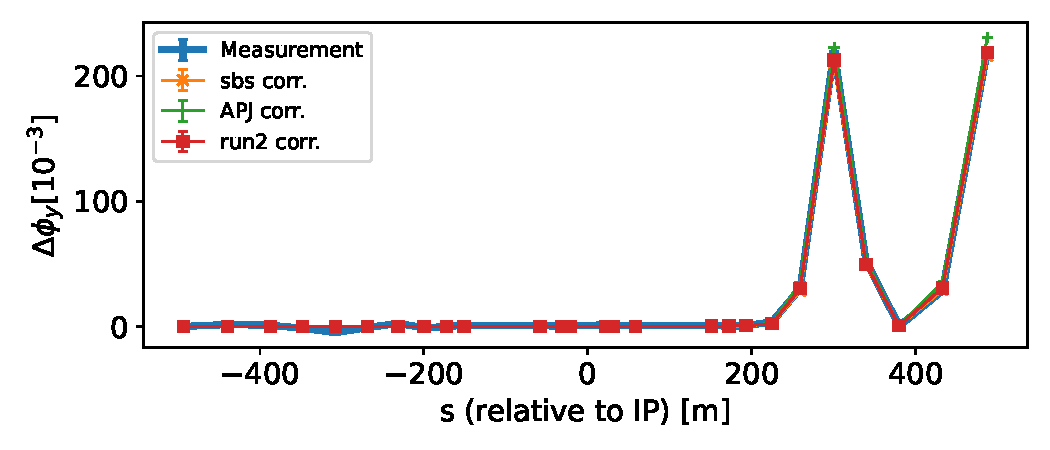
\includegraphics[width=0.4\linewidth]{images/flattop/beam1_y_IP5.pdf}
        }
        \only<3>{
            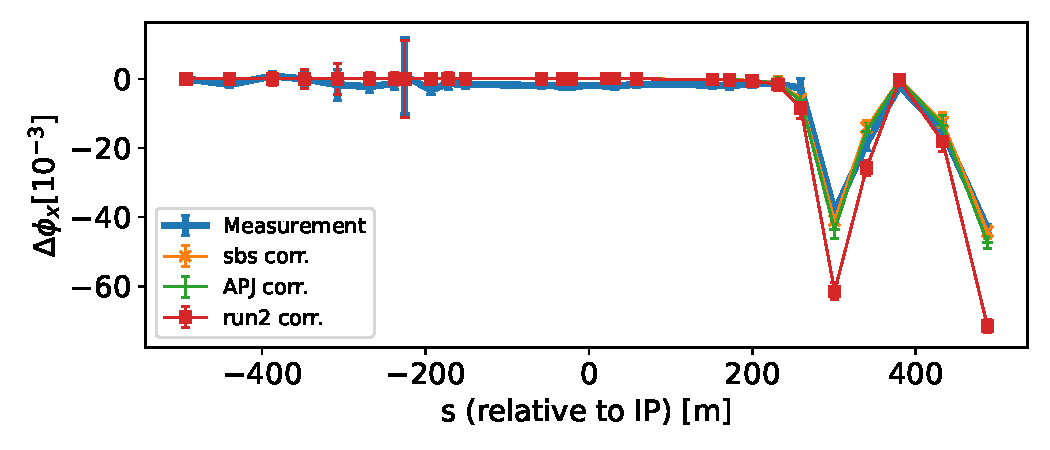
\includegraphics[width=0.4\linewidth]{images/flattop/beam2_x_IP1.pdf}
            \hspace{1cm}
            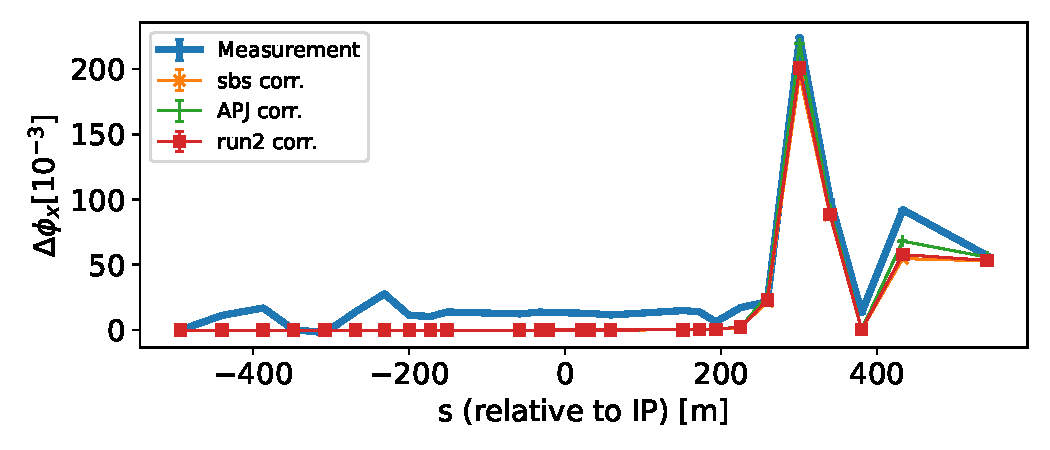
\includegraphics[width=0.4\linewidth]{images/flattop/beam2_x_IP5.pdf}
            \\
            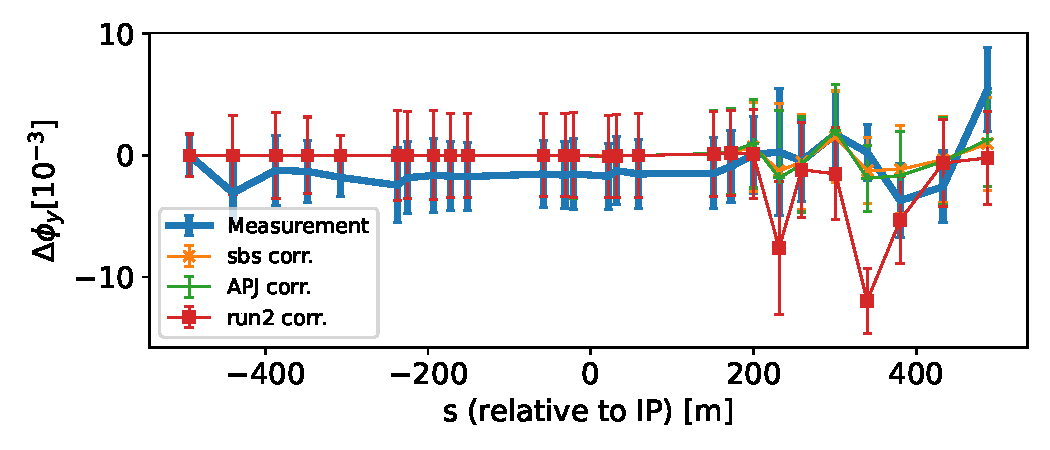
\includegraphics[width=0.4\linewidth]{images/flattop/beam2_y_IP1.pdf}
            \hspace{1cm}
            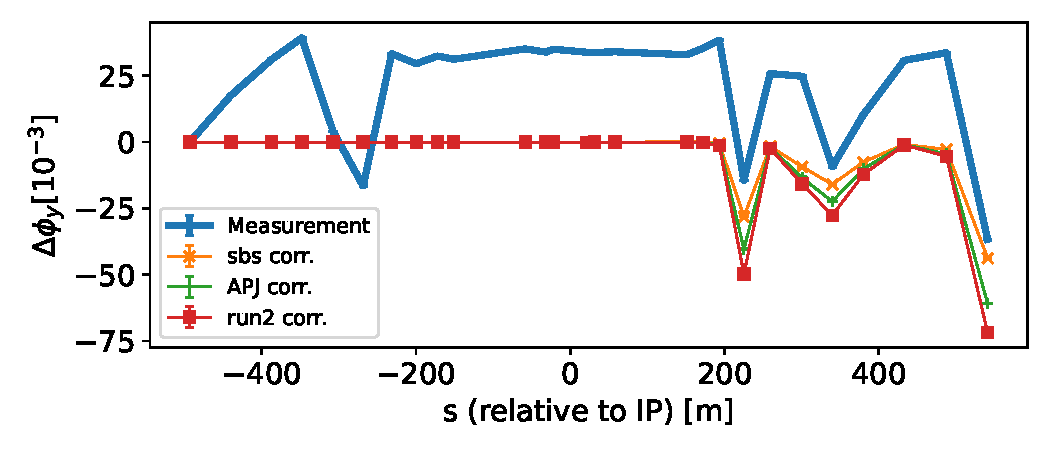
\includegraphics[width=0.4\linewidth]{images/flattop/beam2_y_IP5.pdf}
        }
        \only<1>{
        {\tiny
         \begin{tabular}{l|lSSSS|c|} \toprule
              & \textbf{Circuit}%
              & \multicolumn{4}{c|}{$\Delta k (10^{-5}\SI{}{m^{-2}})$}
              & \textbf{Polarity}%
              \\ \cmidrule{2-6}
              &
              & \multicolumn{1}{c}{\color{RunTwored}\textbf{Run 2}}
              &{\color{APJgreen}\textbf{APJ}}
              &{\color{SbSorange}\textbf{SbS}}
              &{\textbf{ML}}
              & \textbf{LSA} \\\hline \midrule
     IR1 & \texttt{ktqx1.l1} & \color{RunTwored} 1.23 & \color{APJgreen} 0    & \color{SbSorange} 1.23 &  1.23 & - \\
         & \texttt{ktqx1.r1} & \color{RunTwored}-1.23 & \color{APJgreen} 0    & \color{SbSorange}-1.23 & -1.24 & + \\
         & \texttt{ktqx2.l1} & \color{RunTwored} 0.65 & \color{APJgreen} 1.15 & \color{SbSorange} 0.41 & -0.11 & + \\
         & \texttt{ktqx2.r1} & \color{RunTwored}-1.0  & \color{APJgreen}-0.87 & \color{SbSorange}-0.70 &  0.18 & - \\
         & \texttt{ktqx3.l1} & \color{RunTwored} 1.22 & \color{APJgreen} 1.94 & \color{SbSorange} 1.22 &  0.31 & - \\
         & \texttt{ktqx3.r1} & \color{RunTwored}-1.22 & \color{APJgreen}-2.88 & \color{SbSorange}-1.22 & -0.1  & + \\\hline \midrule
     IR5 & \texttt{ktqx1.l5} & \color{RunTwored} 2.0  & \color{APJgreen} 0    & \color{SbSorange} 2.25 & \text{-} & - \\
         & \texttt{ktqx1.r5} & \color{RunTwored}-2.0  & \color{APJgreen} 0    & \color{SbSorange}-2.10 & \text{-} & + \\
         & \texttt{ktqx2.l5} & \color{RunTwored} 0.26 & \color{APJgreen} 0.38 & \color{SbSorange} 0.16 & \text{-} & + \\
         & \texttt{ktqx2.r5} & \color{RunTwored} 1.48 & \color{APJgreen} 0.93 & \color{SbSorange} 1.35 & \text{-} & - \\
         & \texttt{ktqx3.l5} & \color{RunTwored} 1.49 & \color{APJgreen} 3.40 & \color{SbSorange} 2.25 & \text{-} & - \\
         & \texttt{ktqx3.r5} & \color{RunTwored}-1.49 & \color{APJgreen}-2.46 & \color{SbSorange}-2.10 & \text{-} & + \\\hline \midrule
        \end{tabular} 
        }
        }
    \end{center}
    \begin{itemize}
        \item measurements at $\beta^*=\SI{30}{\centi\meter}$ performed
        \item corrections calculated using \highl{APJ}, \highl{SbS}, \highl{ML} and taken from \highl{run2}
        \item ML correction yield good results but are \highl{less local}
        \item APJ and SbS yield \highl{similar corrections},
            run2 corrs are over-correcting
    \end{itemize}
\end{frame}


\begin{frame}{30\,cm Optics -- before and after local corrections}

    \begin{center}
    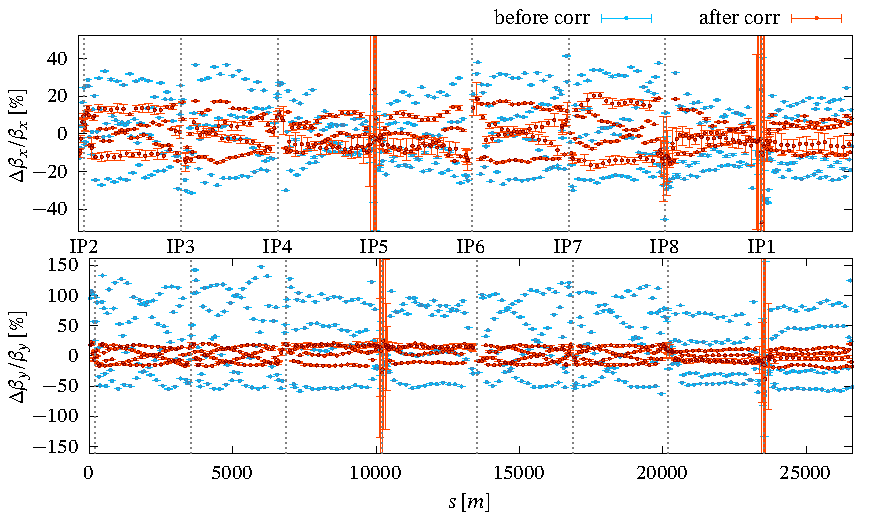
\includegraphics[width=0.49\linewidth]{images/squeeze/b1_bb_comp.pdf}
    \hfill
    
\includegraphics[width=0.49\linewidth]{images/squeeze/b2_bb_comp.pdf}
    \end{center}
    
    \begin{itemize}
        \item $\beta$~beating \highl{after implementation} of local corrections in IPs \textbf{1}, \textbf{2}, \textbf{5} and \textbf{8}
        \item IP1 correction is taken from \highl{APJ}, others from \highl{SbS}
        \item $\beta$~beating stays \highl{under 20\%}
    \end{itemize}
    
\end{frame}


\begin{frame}{30\,cm Optics -- before and after first global corrections}

    \begin{center}
    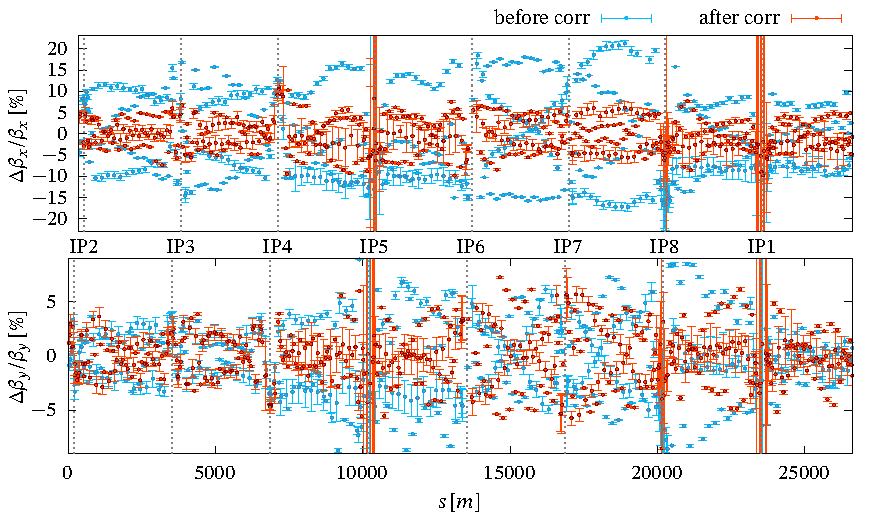
\includegraphics[width=0.49\linewidth]{images/squeeze/b1_bb_comp_after_global.pdf}
    \hfill
    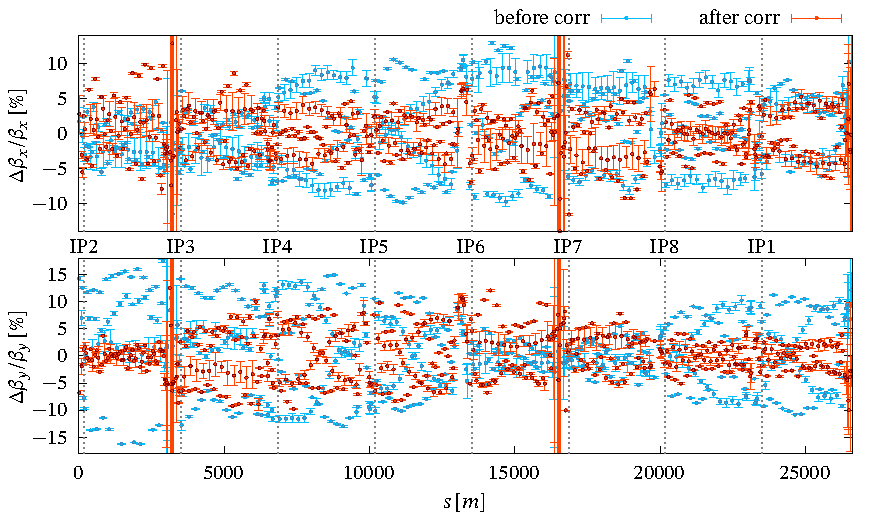
\includegraphics[width=0.49\linewidth]{images/squeeze/b2_bb_comp_after_global.pdf}
    \end{center}
    
    \begin{itemize}
        \item after correction \highl{under 10\,\%} $\beta$~beating
    \end{itemize}
    
\end{frame}

\begin{frame}{Coupling Corrections}
    \begin{minipage}{0.55\linewidth}
        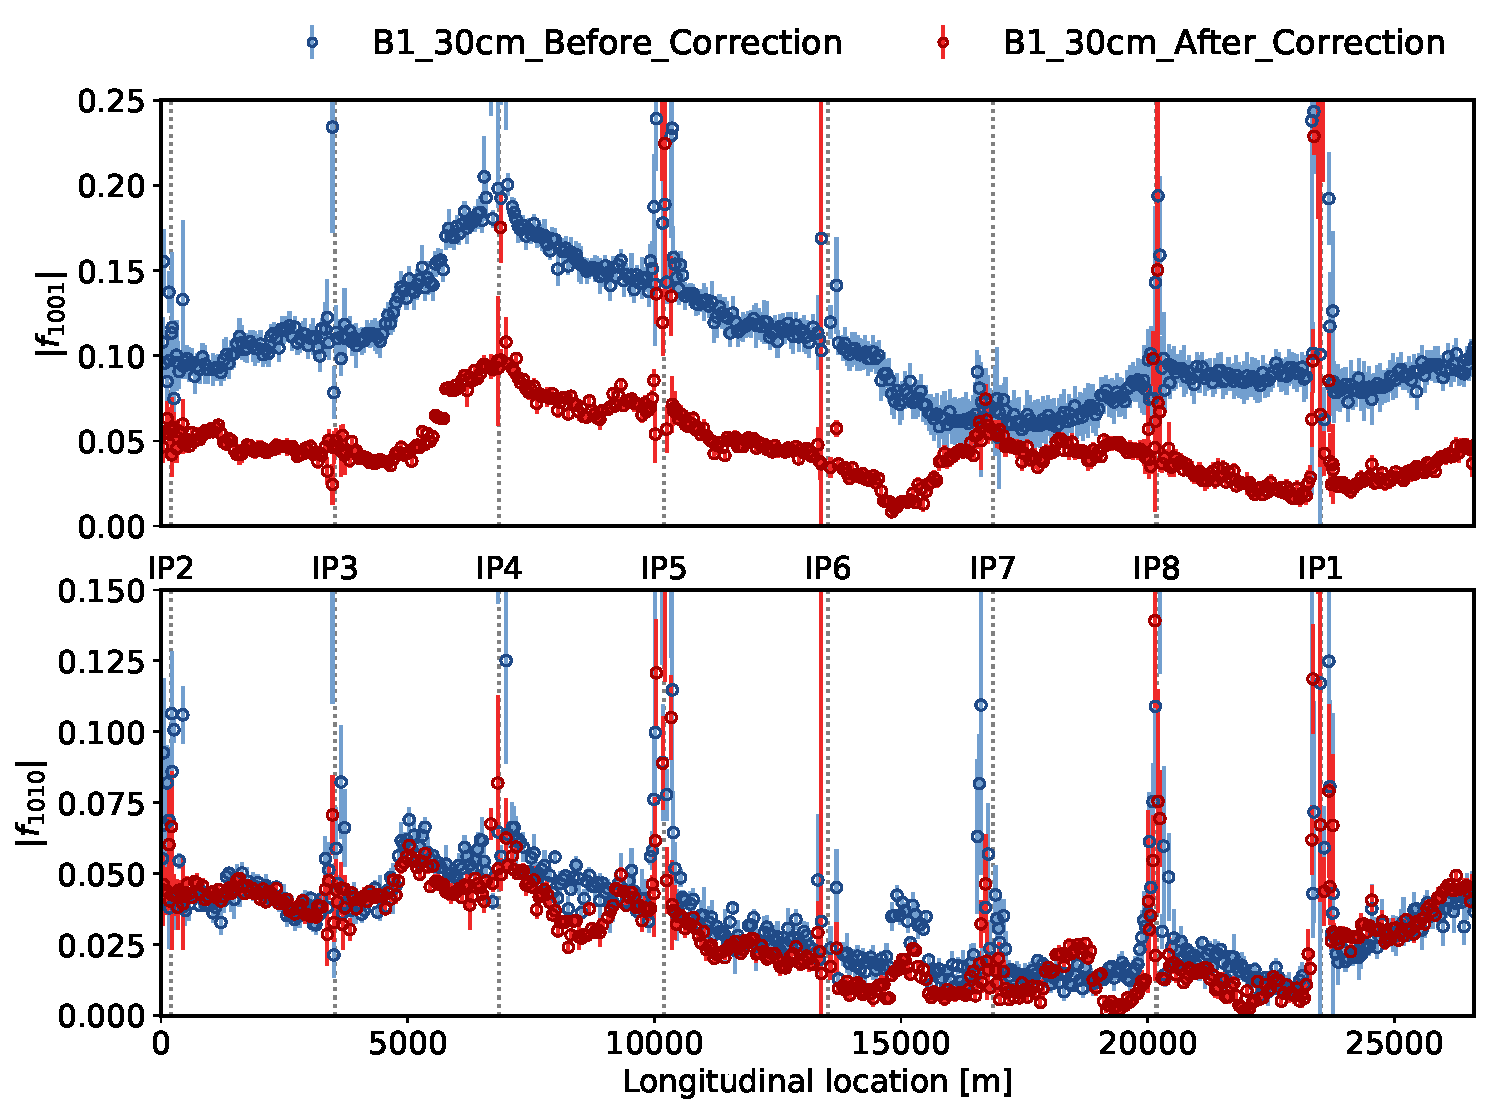
\includegraphics[width=\linewidth]{lhcb1_30cm_before_vs_after_arc_by_arc_coupling.pdf}
    \end{minipage}
    %
    \begin{minipage}{0.44\linewidth}
        \begin{itemize}
            \item local correction in the IPs
            \item B1 arc correction to flatten the coupling structure
            \item new method to find the right balance in the IPs (MQSX) between left and right,
            preliminary analysis indicates that it's close to optimal (IP1)
        \end{itemize}
    \end{minipage}
\end{frame}

%\begin{frame}{K Modulation after global corrections}
%\begin{center}
%   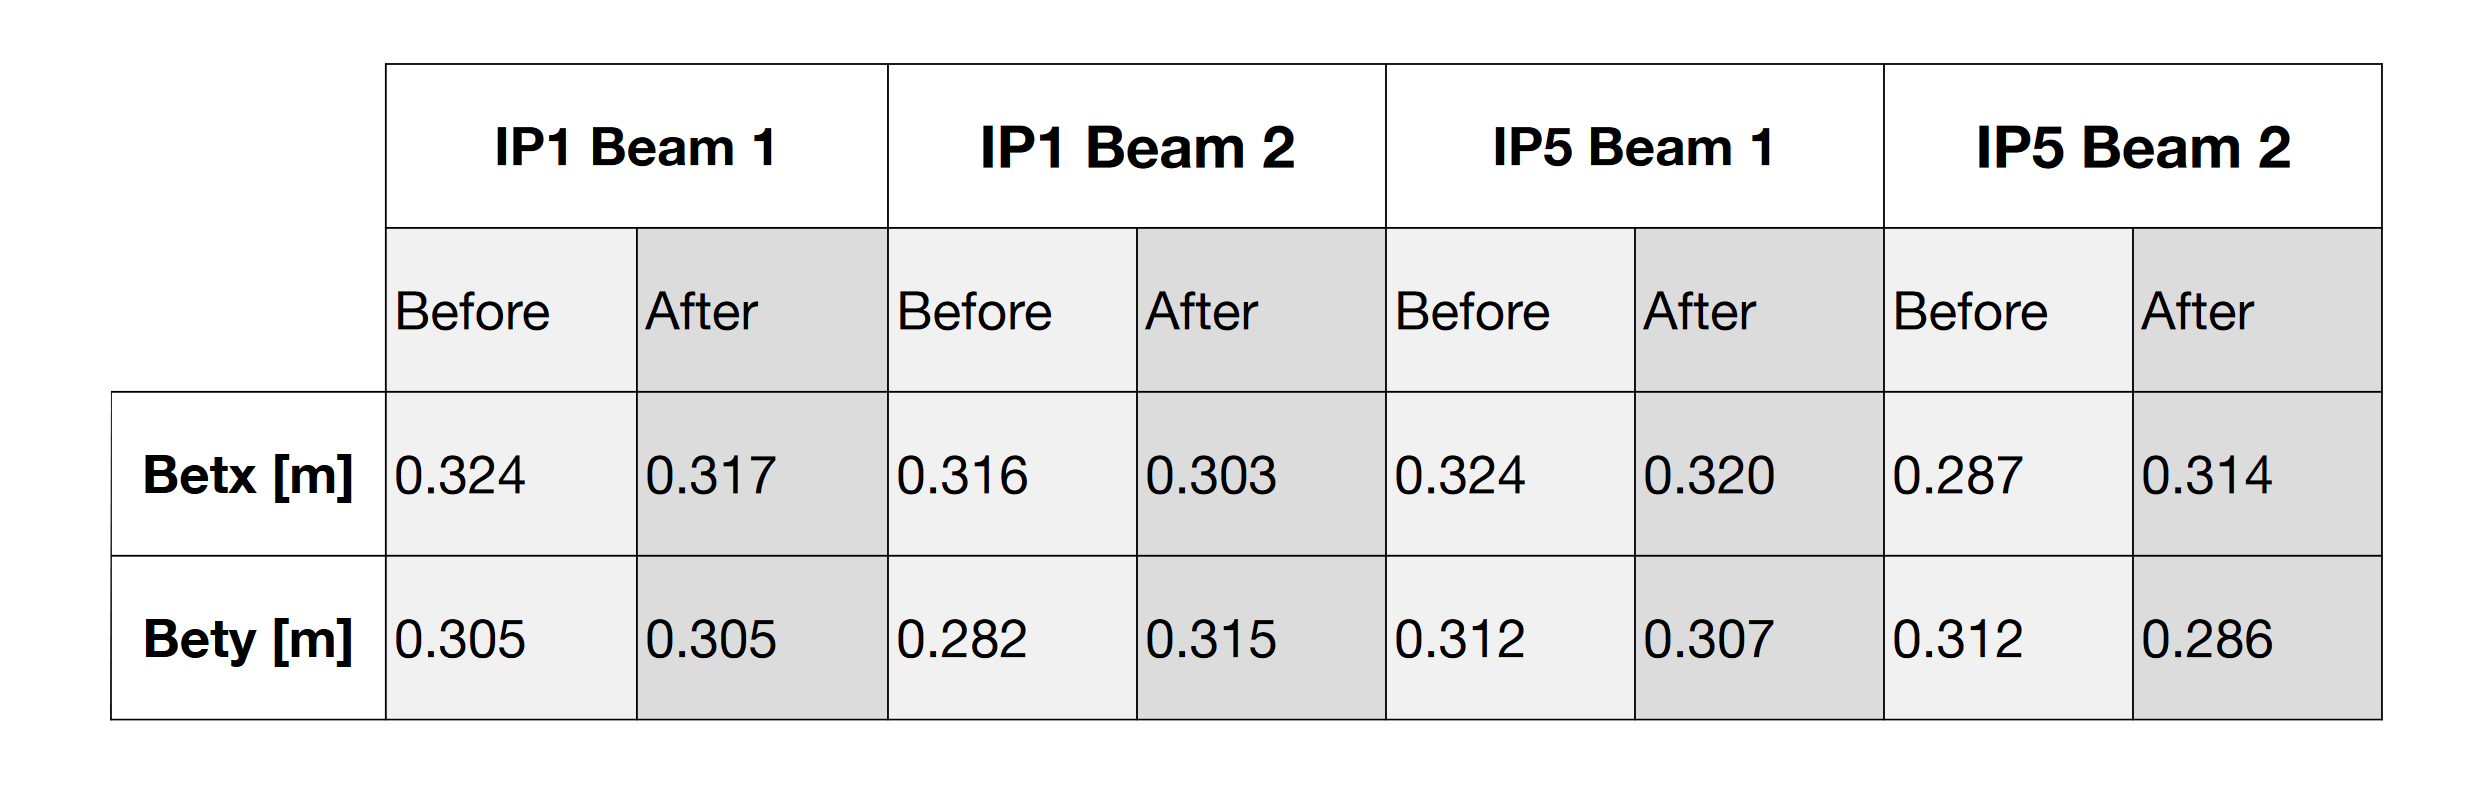
\includegraphics[width=0.7\linewidth]{kmod_after_global.png} 
%\end{center}
%\begin{itemize}
%    \item slight improvement
%    \item still $7\%$ $\beta$~beating at IP5 Beam 1
%\end{itemize}
%\end{frame}


%% Ballistic -------------------------------------------------------------------
%\section{Ballistic}
%\begin{frame}{Ballistic Optics}
%    
%\end{frame}
%
%
% Non-Linear ------------------------------------------------------------------
\section{Non-linear optics}


\begin{frame}{Chromaticity}
    %\begin{center}
    %    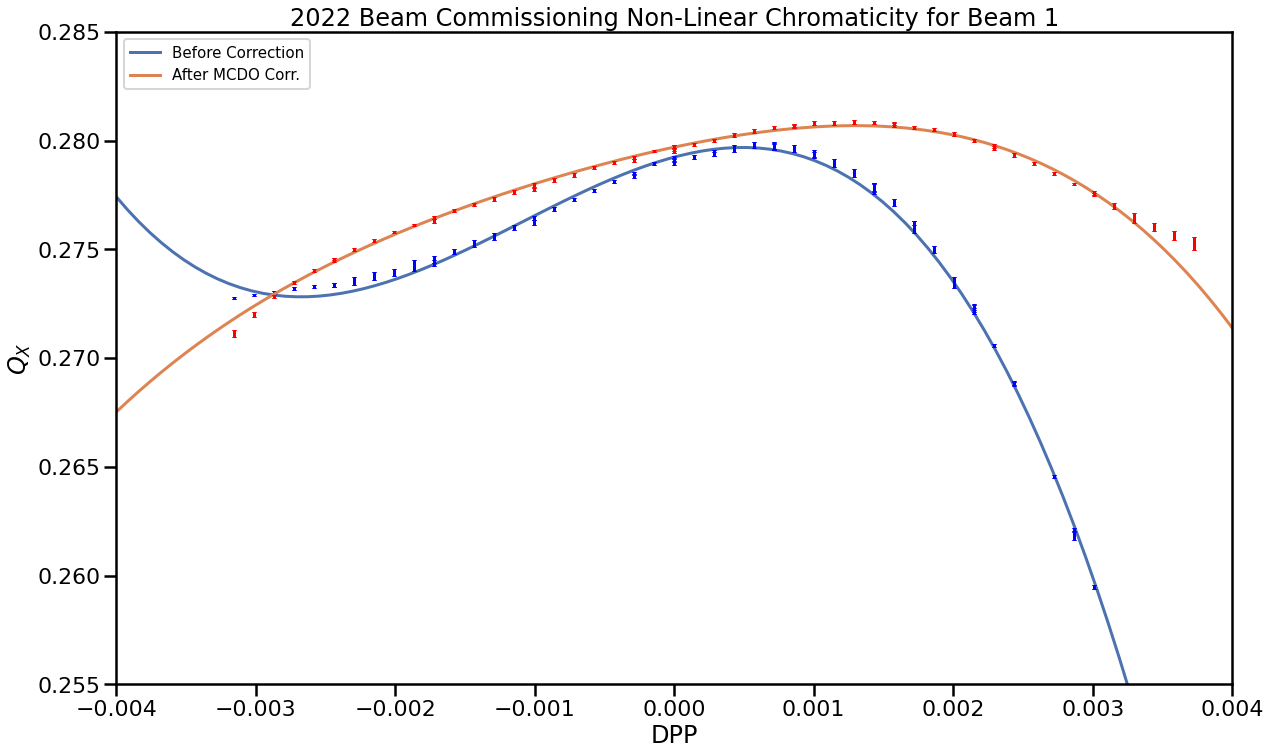
\includegraphics[width=0.49\linewidth]{images/nonlinear/comparison/qxb1q4.png}
    %\end{center}
    \begin{tabular}{l|SS|Sl}
        &\multicolumn{2}{c|}{Beam 1} & \multicolumn{2}{c}{Beam 2}  \\
        &\textbf{injection} & \textbf{60 deg} & \textbf{injection} & \textbf{60 deg} \\ 
        \hline
       $Q''_x\, [10^3]$  & -0.61 \pm 0.013 & -13.22 \pm 1.58 & -0.85 \pm 0.014 & -\\
       $Q''_y\, [10^3]$  & -0.23 \pm 0.012 &   7.83 \pm 0.08 & -0.29 \pm 0.012 & -\\
       $Q'''_x\, [10^6]$ & -1.00 \pm 0.03  & -19.56 \pm 4.73 &  0.66 \pm 0.03  & -\\
       $Q'''_y\, [10^6]$ &  0.13 \pm 0.02  &  12.35 \pm 0.37 &  0.09 \pm 0.02  & -\\
    \end{tabular}\\[1em]
    
    \begin{itemize}
        \item $Q''$ and $Q'''$ \highl{agree} with run II%, $Q'''$ does \highl{not}
        \item \highl{much larger} $dp/p$ range (2015: $\SI{2.5e-3}{}$, now: $\SI{3.5e-3}{}$)
        \item $Q''$ and $Q'''$ \highl{corrected} 
    \end{itemize}
\end{frame}


%\begin{frame}{b5 Resonance}
%    \begin{center}
%        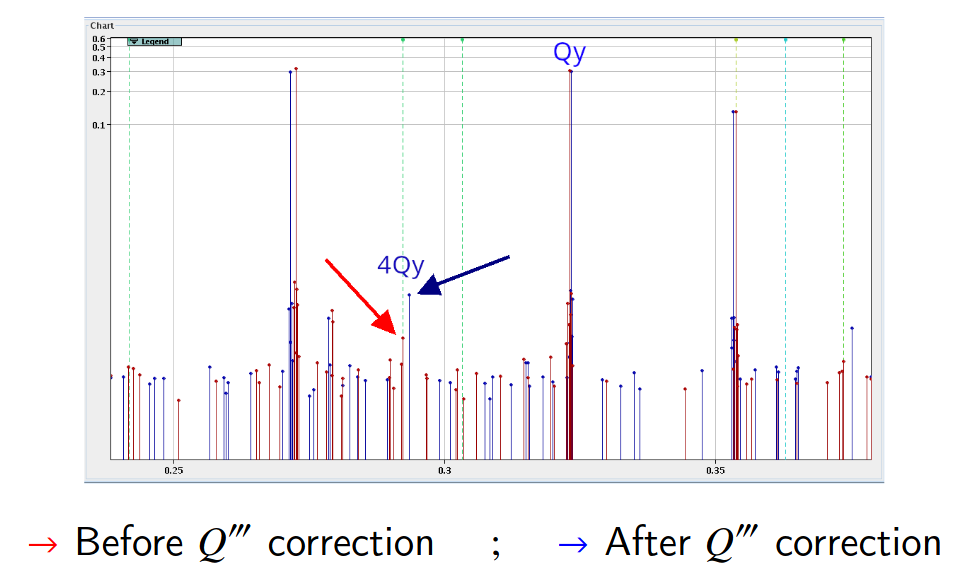
\includegraphics[width=0.5\linewidth]{images/nonlinear/b5_preliminary.png}
%    \end{center}
%    \begin{itemize}
%        \item b5 resonance observed
%        \item seems to get worse after $Q'''$ corrections (non-global source of b5)
%    \end{itemize}
%\end{frame}


\begin{frame}{Amplitude Detuning at $\beta^*$ = 30cm, top energy}
    \begin{center}
        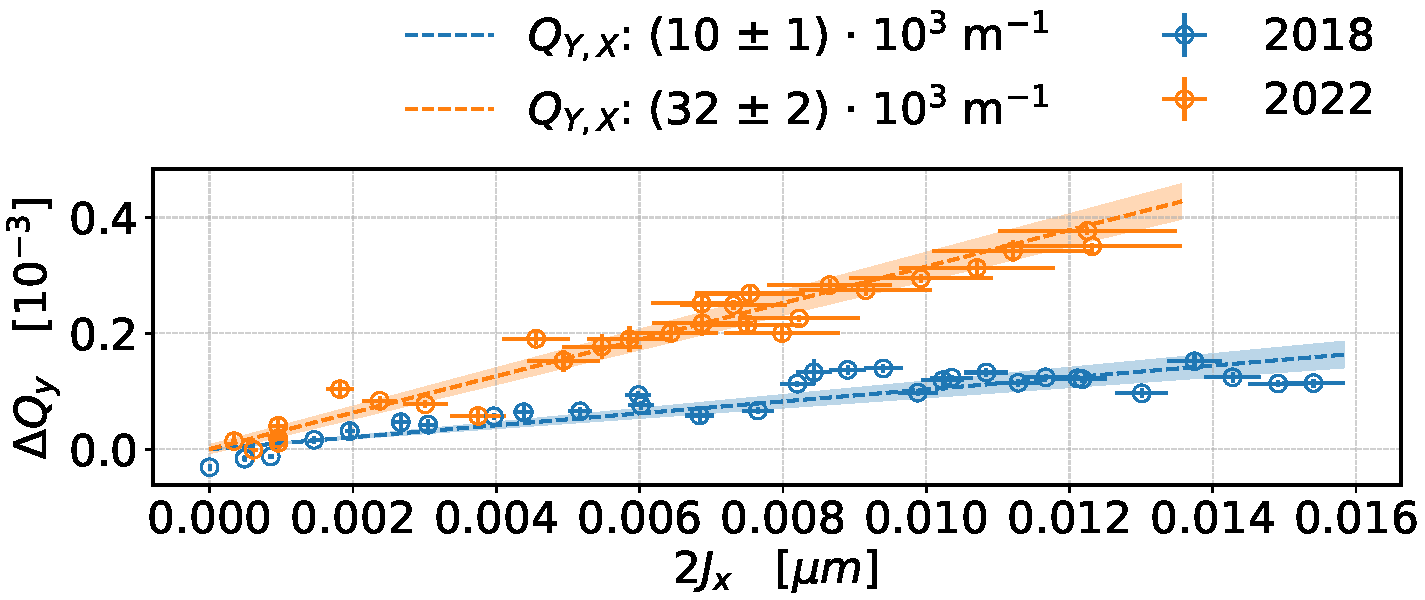
\includegraphics[width=0.5\linewidth]{images/nonlinear/comparison_2018_2022_dQYd2JX_corrected.pdf}
    \end{center}
    
    \begin{itemize}
        \item amplitude detuning \highl{larger} than in run 2
        \item at injection corrected to the level of \highl{previous years}
    \end{itemize}
\end{frame}


\section{Model Creation}

\begin{frame}{Knob extraction}

\begin{itemize}
    \item \highl{past attempts} to introduce an online model \highl{failed}
    \item OMC-OP workshop: decision to create \highl{central optics repository}
    \item  global effort \highl{OP}+\highl{ABP}, combining acc-models (repository of design optics) with
LSA (online information about trimmed-in knobs)
    %\item (TODO: insert sketch of workflow)
    \item still not fully adapted: up to 02.06 trim to wrong place
    %("We all need to get used to this, people are still used to trim everything on correction..." -- Michi)
    \item current status: separate scripts, modular, plan to combine in one repository
\end{itemize}

\end{frame}

\section{Optics Reproducibility}

\begin{frame}{Reproducibility}

    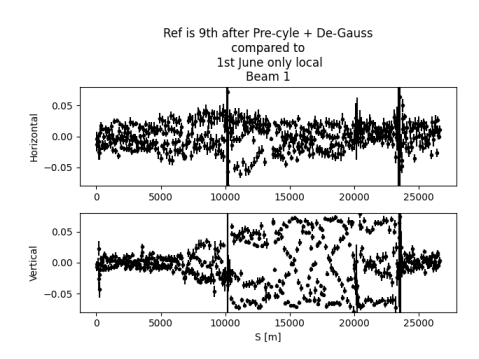
\includegraphics[width=0.45\linewidth]{B1_1June_Ref9May.png}
    \hfill
    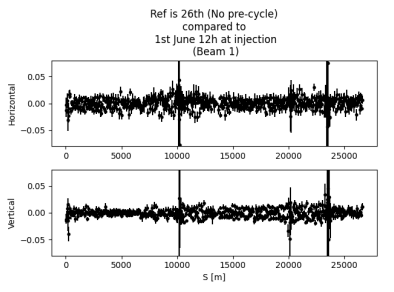
\includegraphics[width=0.45\linewidth]{B1_1June_Ref26May.png}

\only<1>{
\begin{itemize}
    \item  commissioning \highl{robust}, from 26 until today reproducibility \highl{below 2 \%}
    \item  full understanding \highl{ongoing},  will be covered later
\end{itemize}
}

\only<2>{
\begin{itemize}
    \item run3 commissioning features \highl{more techniques} than in run2, e.g.:
    local corrections,
    feed-down from sextupoles in arcs, 
    \item hiccup from changin in $\beta$~beat but \highl{now robust},
    \item are doing \highl{final steps} for commissioning now
    $\Rightarrow$ final configuration that we will \highl{leave in the machine}
\end{itemize}
}
    
    
    
    
    %for stephane: magnetic tcts ruled out 
    
\end{frame}

% \backcover

\end{document}
